\section{Survey Methodology and Results} \label{section:survey-methodology}
	\subsection{Research Design}
		This review is based on a systematic survey of studies primarily done within the period 2019 to 2023. Most recent information has been included for advancement in the field of fashion recommendation and virtual try-on.
	
	\subsection{Search Strategy}
		\textit{Google Scholar} and the \textit{dblp computer science bibliography} have been instrumental in providing results for searches using important keywords like, `artificial intelligence, augmented reality, clothing, fashion, recommendation, computer vision, and virtual try-on.'

	\subsection{Inclusion \& Exclusion Criteria}
		The survey was conducted with the following inclusion criteria:
		\begin{enumerate}
			\item Does the study deal with the use of technologies in fashion for recommenders and virtual try-on?
			\item Is the study comparable to existing state-of-the-art techniques?
		\end{enumerate}
	
	\subsection{Survey Results}
		147 documents were included in the final collection for analysis. Figure \ref{fig:document-collection} illustrates the flow of the collection process, and Figure \ref{fig:document-domains} shows the distribution of the collected documents per domain.

	\begin{figure}
		\centering
		\begin{tikzpicture}[
			node distance=10mm and 5mm,
			start chain=going below,
			rNode/.style = {
				draw, rectangle, align=center, text width=2.75cm,
				font=\small, inner sep=2.5mm, outer sep=0pt,
				on chain},
			mylabel/.style = {
				draw, rectangle, align=center, rounded corners, 
				font=\small\bfseries, inner sep=2.5mm, outer sep=0pt,
				fill=black!5, minimum height=30mm,
				on chain},
			every join/.style = arrow,
			arrow/.style = {very thick,-stealth}
		]
			\node (n1) [rNode] {957 documents found using keywords};
			\node (n2) [rNode, join] {209 additional documents identified  through other sources};
			\node (n3) [rNode, join] {1064 full-text articles assessed for eligibility};
			\node (n4) [rNode, join] {137 documents included in survey};
			\node (n1r) [rNode, right=of n1] {883 documents after duplicates removed};
			\node (n2r) [rNode, right=of n2] {28 documents excluded};
			\node (n3r) [rNode, right=of n3] {927 documents excluded:\\
				Not relevant: 791 \\
				Not SOTA: 136
			};
			\draw[arrow] (n1) -- (n1r);
			\draw[arrow] (n2) -- (n2r);
			\draw[arrow] (n3) -- (n3r);
			\begin{scope}[node distance=2.5mm]
				\node[mylabel,below left=-3mm and 4mm of n1.north west, minimum height=20mm] {\rotatebox{90}{Identification}};
				\node[mylabel, minimum height=25mm] {\rotatebox{90}{Screening}};
				\node[mylabel, minimum height=21mm] {\rotatebox{90}{Eligibility}};
				\node[mylabel, minimum height=19mm] {\rotatebox{90}{Included}};
			\end{scope}
		\end{tikzpicture}
		\caption{Document collection flowchart}
		\label{fig:document-collection}
	\end{figure}

	\begin{figure}
		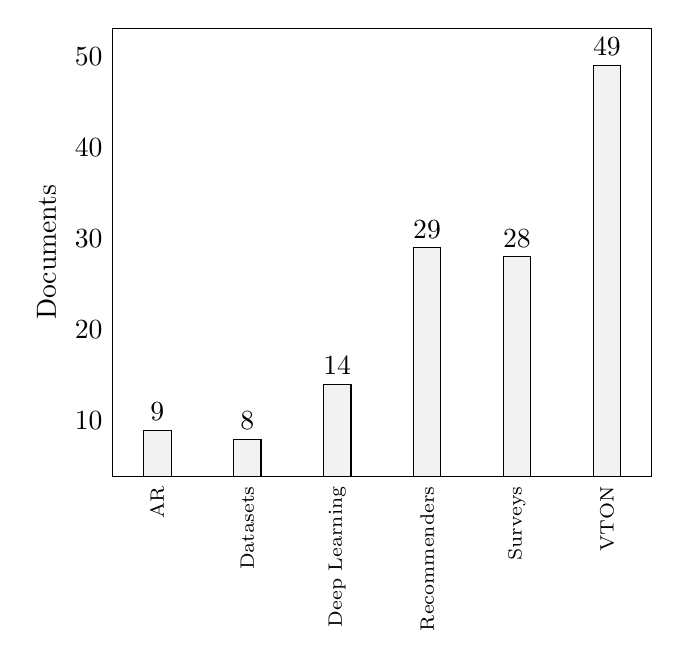
\begin{tikzpicture}
			\begin{axis}[
				symbolic x coords={AR, Datasets, Deep Learning, Recommenders, Surveys, VTON},
				ylabel = {Documents},
				xticklabel style = {font=\scriptsize, anchor=east, rotate=90},
				xtick=data,
				nodes near coords,
				tick style={draw=none}
			]
				\addplot[ybar, fill=black!5] coordinates {
					(AR, 9)
					(Datasets, 8)
					(Deep Learning, 14)
					(Recommenders, 29)
					(Surveys, 28)
					(VTON, 49)
				};
			\end{axis}
		\end{tikzpicture}
		\caption{Document domain distribution}
		\label{fig:document-domains}
	\end{figure}

	% Total papers:

	% Fashion (957)
	% 	2023 (155)
	% 	2022 (211)
	% 	2021 (193)
	% 	2020 (190)
	% 	2019 (208)
	% Recommenders (116)
	% 	2023 (13)
	% 	2022 (29)
	% 	2021 (18)
	% 	2020 (21)
	% 	2019 (35)
	% VTON (200)
	% 	2023 (36)
	% 	2022 (66)
	% 	2021 (49)
	% 	2020 (22)
	% 	2019 (27)